\newpage

\section*{\centerline{Цель работы}}

Получение навыков работы с командной строкой UNIX и UNIX-подобных систем, а также навыки работы с каталогами, папками и дисками в GNU/Linux. Изучить основные команды и утилиты GNU/Linux. 

\newpage
\section*{\centerline{Выполнение}}

\subsection*{Задание 1.2}
	\paragraph{1)}
	При помощи команды \textit{pwd} можно определить абсолютный путь до текущего расположения. При помощи команды \textit{mkdir} мы создаем пустую папку. C помощью команды \textit{cd} можно перемещаться по директориям.\\
	\\
	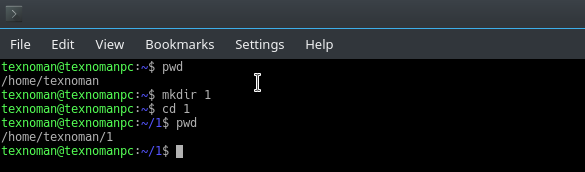
\includegraphics[width=\textwidth]{1.png}




